\documentclass[12pt,a4paper]{report}
%\fontencoding{T1}

\usepackage[utf8]{inputenc}
\usepackage[T1]{fontenc}
\usepackage[danish]{babel}
\usepackage[hidelinks]{hyperref}
\usepackage{lingmacros}
\usepackage{tree-dvips}
\usepackage{url}
\usepackage{array}
\usepackage{graphicx}
\usepackage{float}
\usepackage{rotating}
\usepackage{lastpage}
\usepackage{color}
\usepackage[x11names,rgb,usenames,dvipsnames,svgnames,table]{xcolor}
\usepackage{colortbl}
\usepackage{algorithm2e}
\usepackage{geometry}
\usepackage{listings}
\usepackage{titlesec, blindtext, color}
\definecolor{gray75}{gray}{0.75}
\definecolor{gray90}{gray}{0.90}
\definecolor{ForestGreen}{RGB}{15,116,61}
\definecolor{ForestLight}{RGB}{57,181,74}
\definecolor{ForestDark}{RGB}{0,104,56}
\definecolor{Sapphire}{RGB}{28,117,188}
\definecolor{gray25}{gray}{0.25}
\newcommand{\hsp}{\hspace{20pt}}

\usepackage{tikz}
\usetikzlibrary{snakes,arrows,shapes}
\usepackage{amsmath}

\usepackage{xcolor} 
\usepackage{fix-cm} 
\usepackage{pgfplots}

%Titelblad fix
%\usepackage[ansinew]{inputenc}
\usepackage{a4}

\titleformat{\chapter}[hang]{\Huge\bfseries}{\thechapter\hsp\textcolor{gray75}{|}\hsp}{0pt}{\Huge\bfseries}

\begin{document}
\setcounter{page}{2}

\begin{titlepage}
\newcommand{\HRule}[1]{\hfill \rule{0.2\linewidth}{#1}} 

\definecolor{grey}{rgb}{0.9,0.9,0.9} 
\newgeometry{top=1.5in,bottom=1in,right=0cm,left=0cm}
\thispagestyle{empty} 
\centering {\LARGE Aalborg Universitet}
\vspace*{1.5cm}

\noindent \colorbox{Sapphire}{
	 \parbox[t]{1.0\linewidth}{
		\centering \fontsize{50pt}{80pt}\selectfont
		\vspace*{1.0cm}
        \textcolor{White}{
        \sffamily{
		SMS Komprimering \\[3pt]
        %\LARGE Komprimering af korte beskeder \\ 
        }
		\vspace*{0.7cm}
        }
	}
}
\\[2em]
\huge P1-Projekt

\vfill
\flushright
\flushright \rule[20pt]{0.1pt}{9em}  \begin{minipage}[b]{0.50\linewidth}
{
\Large
\textbf{Gruppe B228:} \\
    Bossen, Jannek Alexander Westerhof\\
    Brämer, Kevin\\
    Bønneland, Frederik Meyer\\
    Joensen, Ólavur Debes\\
    Olesen, Anders Trier\\
    Tjell, Katrine Sofie\\
}
\end{minipage}
\clearpage 

\thispagestyle{empty}
\end{titlepage}

%create empty page
\newpage
\thispagestyle{empty}
\mbox{}

%Hent titelblad (Som henter synopsis fra Indhold/Synopsis.tex):
\begin{titlepage}
\begin{nopagebreak}
{\samepage 
\begin{tabular}{r}
\parbox{\textwidth}{  \raisebox{11mm}{\includegraphics[height=1.2cm]{Billeder/aau-logo.pdf}}
\hfill \parbox{4.9cm}{\begin{tabular}{l}
{\sf\small \textbf{Det Teknisk-Naturvidenskabelige Basis{\aa}r }}\\
{\sf\small  \textbf{Elektronik og Elektroteknik}} \\
{\sf\small Strandvejen 12-14} \\
{\sf\small Telefon 96 35 97 31} \\
{\sf\small Fax 98 13 63 93} \\
{\sf\small http://tnb.aau.dk}
\end{tabular}}}
\\
\end{tabular}

\begin{tabular}{cc}
\parbox{7cm}{
\begin{description}

\item {\bf Titel:} 

skriv her
  
\item {\bf Tema:} 

Virkelighed og modeller

\end{description}

\parbox{8cm}{

\begin{description}
\item {\bf Projektperiode:}\\
   P1, efter{\aa}rssemesteret 2004\\
  \hspace{4cm}
\item {\bf Projektgruppe:}\\
  skriv her\\
  \hspace{4cm}
\item {\bf Deltagere:}\\
skriv her \\
skriv her \\
skriv her \\
skriv her \\
skriv her \\
skriv her \\
  \hspace{2cm}
\item {\bf Vejledere:}\\
 skriv her \\
  skriv her \\
\end{description}
}
\begin{description}
\item {\bf Oplagstal:} ??
\item {\bf Sidetal:} ??
\item {\bf Bilagsantal og --art:} ??
\item {\bf Afsluttet den} ??
\end{description}
\vfill } &
\parbox{7cm}{
  \vspace{.15cm}
  \hfill 
  \begin{tabular}{l}
  {\bf Synopsis:}\bigskip \\
  \fbox{
    \parbox{6.5cm}{\bigskip
     {\vfill{\small Dette projekt handler om komprimering af SMS-beskeder. Problemstilling i projeket er, at en SMS-besked har en begrænsning på 160 tegn og hvis denne begrænsning overskrides betales der SMS-takst for hver påbegyndt besked. I rapporten undersøges hvilke løsninger der allerede findes og det diskuteres hvem der kunne være interesseret i en løsning på problemet. Udover rapporten er der udarbejdet et program som kan komprimere og dekomprimere en tekstbesked, hvorved det bliver muligt at sende flere tegn i samme SMS. Herved kan vi konkludere at det er muligt at sparer brugeren for dobbelt SMS-takst ved at komprimere SMS-beskeder inden afsendelse.
     \bigskip}}
     }}
   \end{tabular}}
\end{tabular}}
\\ \\
\noindent{\footnotesize\emph{Rapportens indhold er frit tilg�ngeligt, men offentligg�relse (med kildeangivelse) m� kun ske efter aftale med forfatterne.}}
\end{nopagebreak}
\end{titlepage}

%create empty page
\newpage
\thispagestyle{empty}
\mbox{}
\addtocontents{toc}{\protect\enlargethispage{\baselineskip}}
{\small\tableofcontents}
% Fjerner sidetal på indholdsfortegnelse
\thispagestyle{empty}
\renewcommand{\chaptername}{Kapitel}


%create empty page
\newpage
\thispagestyle{empty}
\mbox{}

% TEKST SÆTTES UNDER HER
\chapter{Indledning}
\setcounter{page}{3}
	I 1992 blev den første SMS afsendt \cite{museum}. Dengang kunne denne type tekstmeddelse maksimalt rumme 160 tegn, hvilket er nøjagtig lige så mange tegn, som en SMS kan indeholde i dag. Det var den tyske enginør Friedhelm Hildebrand, der i 1985 så potentialet i muligheden for at sende korte tekst beskeder fra mobiltelefon til mobiltelefon. Han undersøgte, hvor mange tegn der normalt blev brugt når man skrev et postkort, ligesom at han selv skrev forskellige beskeder, som han forestillede sig, at folk ville skrive til andre via deres mobiltelefon. I ingen af tilfældende var antallet af tegn i beskederne over 160. Derfor blev grænsen for hvor mange tegn en SMS kan indeholde sat ved 160.
Gennem tiden har meget teknologi ændret sig, så måske burde man i dag have muligheden for at sende flere end 160 tegn i en SMS. \cite{hillebrand}

\subsubsection {Datakomprimering}

Datakomprimering handler om at gøre en datamængde mindre. Der kan både være tale om filer, billeder, film osv.. Man ønsker ofte at data skal fylde så lidt som muligt, derfor er komprimering et meget centralt emne indenfor datalogi. Når man eksempelvis taler om hukommelseslager, computernetværk, herunder især internettet, er det meget relevant at data fylder så lidt som muligt.
 
Man kan komprimere enkelte filer såvel som hele samlinger af filer. Mange siger ofte at filer pakkes, når man komprimerer. Der findes allerede flere komprimeringsprogrammer; zip, jpeg, WinZip, SMS ZIP, SMS ZIPPER, for bare at nævne nogle få.

Der findes selvfølgelige mange måder at komprimere på og lige så mange forskellige komprimeringsalgoritmer. Disse algoritmer kan deles op i to kategorier, tabsfri og ikke-tabsfri.  
Det man ofte udnytter når man komprimerer tabsfrit, er at de fleste mængder af data indeholder den samme information flere gange. Eksempelvis indeholder en tekstfil de samme ord gentagne gange. Derfor kan man i stedet for den gentagne information, skrive informationer om hvor mange gange den bestemte information er blevet gentaget. På den måde kan dataene genskabes uden tab. Denne kategori benyttes især til tekstfiler, hvor det er særlig vigtigt at filen kan genskabes 100 procent. Ikke-tabsfri kompression kan eksempelvis benyttes til billedkomprimering, hvor det kan gå an at ikke hver pixel genskabes 100 procent.
 %Indhold af Indledning.tex bliver sat ind her.
	
	\section{Initierende problem}
	Der er forskellige tjenester der giver mulighed for at skrive korte tekstbeskeder. Fælles for dem alle er at det kun er tilladt at skrive et begrænset antal tegn pr. besked, hvis denne grænse overskrides deles beskeden i to. Problemet er, at hvis der eksempelvis er tal om en SMS-besked, kommer man til at betale dobbelt SMS-takst, hvis beskeden bliver delt i to.

\chapter{Analyse}
 
    Dette kapitel beskriver den baggrundsviden, der er nødvendig for at forstå projektet. Bl.a. gives en beskrivelse af hvad GSM er og hvordan SMS-teknologien fungerer, ligesom forskellige komprimeringsalgoritmer introduceres. Sidst i kapitlet fremgår problemformuleringen for projeket, efterfulgt af kravene til det udarbejdet produkt.

    \section{GSM}
    I 1982 begyndte man at arbejde på et ”anden generations”(2G) system indenfor mobiltelefoni og kaldte det for ”Groupe Spécial Mobile”(GSM). Inden da havde telekommunikation foregået analogt, og sådan blev det ved indtil 1991, hvor denne digitale form for mobiltelefoni, GSM, blev sat i gang. Systemet blev hurtigt internationalt udbredt, og man besluttede sig for at omdøbe det til ”Global System for Mobile communications”. Det er dog aldrig blevet til et globalt system, idet man i Japan og USA bruger andre systemer \cite{denstoredanske}.

GSM netværket består af forskellige celler, som hver har en basestation, der kan modtage og sende signaler, se figur \ref{celler}. Basestations-controlleren, som ses på figur \ref{celler}, er ansvarlig for radioressourcer for en eller flere basestationer. Basestations-controlleren har forbindelse til "mobile switching center", som er netværksenheder, der tager sig af den trådløse kommunikation. Basestationer dækker, med deres individuelle radius, hver især et geografisk område, altså en celle. Jo mindre radius en basestation har, jo større er dens tilgængelige båndbredde. Stationer som dækker byområder, kan derfor have en radius på helt ned til få hundrede metre mens stationer, som står længere ude på landet kan dække en radius på op til 30 kilometer. \cite{techviral}

\begin{figure}[H]
\centering
\includegraphics []{Billeder/celler.png}
\caption {Celler, som hver dækker deres eget geografiske område \cite{techviral}}
\label {celler}
\end{figure} 

Når man bruger sin mobiltelefon vil den, gennem luften, skabe kontakt til den nærmeste basestation. Hvis man har sendt en SMS-besked, vil denne modtages af basestationen, som sender den videre til SMS-centeret. Som det ses på figur \ref{GSM}, vil SMS'en inden den kommer til SMS-centeret, gå igennem mobile switching ceter, som giver den ruteoplysninger, så den kan nå frem til modtageren. SMS-centeret er herefter ansvarlig for at viderebringe SMS’en til modtageren. Hvis SMS-centeret ikke kan få forbindelse til modtagertelefonen (hvis denne er slukket eller udenfor signal), gemmes beskeden i centeret og sendes når der er oprettet forbindelse til modtageren. \cite{info}

\begin{figure}[H]
\centering
\includegraphics []{Billeder/GSMnetvaerk.png}
\caption {SMS'ens vej fra afsender til modtager \cite{info}}
\label {GSM}
\end{figure} 

I GSM er der indbygget to muligheder for at sende en anden person flere SMS-beskeder i sammenhæng. Den ene mulighed er SMS-sammenkædning, hvilket vil sige at en række SMS-beskeder bliver kædet sammen og sendes hver for sig, men hos modtageren bliver de sat sammen i korrekt rækkefølge og læses igen som én besked. Den anden mulighed er komprimering af tekst med Huffman coding \cite{UNI}. Hvis denne mulighed udnyttes kan man sende op til 80 tegn mere pr. SMS-besked. Dette kræver dog at telefonen fra fabrikkens side har sprogspecifikke kompressionsparametre. Det har ikke været muligt at finde ud af om man idag reelt gør brug af denne mulighed for at komprimere tekstbeskeder. 


	\section{SMS-teknologi}
	Langt de fleste mennesker besk�ftiger sig dagligt med SMS'er - dog uden at vide hvad der i virkeligheden sker n�r der sendes en SMS. Selv n�r en mobiltelefon ikke er i brug, sender og modtager den sm� datapakker til/fra mobilcentralen. Disse data hj�lper blandt andet med at lokalisere de signalt�rne mobilen er tilkoblet til. Dette kan is�r blive nyttigt, idet at mobilcentralen ved hvilke t�rne der skal benyttes da telefonen skal modtage opkald eller data, som f.eks. SMS'er.

N�r en SMS besked bliver sendt fra en mobil bliver den i f�rste omgang sendt til mobilcentralen via signalt�rne. N�r mobilcentralen modtager beskeden bliver den overf�rt til et SMS-Center (SMSC). SMS-Centeret tager sig af at sende beskeden til den rette modtager, ved at overf�re den til den �nskede modtagers SMS-Center. N�r beskeden n�r frem til den p�g�ldendes center, bliver den, hvis det er muligt, overf�rt til mobilcentralen der sender beskeden til modtageren. Hvis modtageren af en eller anden �rsag ikke er at finde p� et mobilt netv�rk bliver beskeden opbevaret p� SMS-Centeret i op til flere dage, og vil f�rst blive afsendt n�r der er mulighed for det. SMS-Centeret kan endvidere sende en bekr�ftelse til afsenderen, n�r beskeden bliver leveret til modtageren. Alt dette er muligt via Signaling System no. 7 - som er en protokol suite, der indeholder forskellige protokoller. Protokollerne benyttet af SMS systemer befinder sig i mere specifikt i SS7 suitens Mobile Application Part (MAP).

\noindent
\includegraphics[width=\linewidth]{Billeder/Mobil.png}

Signalerings systemerne i MAP er efter design begr�nset til visse st�rrelser af data. Opfinderne af SMS systemet pr�vede med forskellige beskeder, hvorefter man fandt ud af at langt de fleste var under 160 tegn. Man mente derfor at 160 tegn var rigeligt til at rumme de fleste beskeder, og en SMS beskeds maksimale st�rrelse blev derfor defineret til 160 tegn. Efter introduktion af udvidede tegns�t er definitionen pr�ciseret til 140 okteter(bytes), eller 1120 bits. \cite{sms_max1} \cite{sms_max2}.


Da begr�nsningen er defineret i bits, er beskedens maksimale l�ngde afh�ngig af det anvendte tegns�t. Det mest basale er det grundl�ggende 7-bit GSM alfabet. Dette alfabet benytter 7-bits til at symbolisere tegn, hvilket udg�r 128 forskellige muligheder. 7-bit GSM alfabetet begr�nser derfor en SMS beskeds l�ngde til 1120/7 bits = 160 tegn. N�r der er brug for mere avancerede specialtegn, bruger SMS systemer UCS-2 tegns�ttet. Dette tegns�t benytter 2 okteter - alts� 16 bits - til repr�sentation af �t tegn. Ved brug af dette tegns�t mindskes den maksimale l�ngde derfor ned til 1120/16 = 70 tegn.

Enhver SMS-besked indeholder ogs� en header, som der er afsat plads til udover de 140 okteter. En SMS-header indeholder typisk data som f.eks. afsenderens telefonnummer, l�ngden af beskeden, benyttet tegns�t og lignende. Hvis en SMS besked bliver l�ngere end gr�nsen ved det benyttede tegns�t bliver beskeden delt op i flere beskeder. N�r en besked bliver delt op, skrives der information til fletning af beskeden i headeren - og da der ikke er afsat plads til ekstra header information, bliver der brugt 6 okteter af de oprindelige 140 i beskeden. Dette begr�nser l�ngden yderligere til 153 ved 7-bit encoding og 67 ved 16-bit encoding.
	
	\section{Tegnsæt}
	For at kunne komprimere en besked er det vigtigt at kende til teknologien bag sms’er.

Den teknologi som anvendes i moderne telefoner hedder GSM (Global System for Mobile Communications), som er en 2G standard.# Denne teknologi gør det muligt at benytte sig af sms’er.\cite{GSM_term}

For at et computersystem skal have muligheden for at kunne printe tegn til skærmen, er det nødvendig at repræsentere disse tegn med hver sit tal. Disse tal har man bestemt i en standard, som betyder at alle skal benytte de samme tal, for de samme tegn, og derved gøre det lettere for programmørerne af softwaren der benytter disse tegn. Den mest brugte standard indenfor tegnsæt, som dette kaldes, er unicode.\cite{UNICODE_standard}

I mobiler der gør brug af GSM, kan der til sms’er, benyttes et tegnsæt kaldt GSM 03.38. Dette tegnsæt kan kodes i en række alfabeter, hvor standard alfabetet GSM 7 bit er et krav ved skabelse af mobiltelefoner.\cite{GSM_7_bit]

Nedenunder ses et skema af GSM 7 bit alfabetet:
	
	\section{Komprimeringsalgoritmer}
	\subsection{Entropikodning}
Entropikodning er en lossless/tabsfri datakomprimeringsmetode. Tabsfri, betyder at der ikke går nogen information tabt, ved at komprimere datamængden. Modsat har vi lossy/tabsgivende komprimering, som fx MP3, og JPEG. Entropopikodning går ud på, at få en given datamænde til at benytte et minimalt antal bit. Dette kan opnås ved at kigge på hyppigheden af de forskellige tegn i datamængden, der skal komprimeres, og give de oftest fremkommende symboler få bits, og de mere sjældne symboler flere bits. Formålet er, at få det gennemsnitlige antal bits pr. symbol(middelkodelængden) ned. Den teoretiske nedre grænse for middelkodelængden kaldes datamængdens entropi. \cite{entro1}
Der findes flere forskellige entropikodningsmetoder, og et par eksempler er "Huffman kodning" og "arithmetic coding".


\subsection{Huffman Coding}
Komprimeringsalgoritmen "Huffman coding", er udviklet af David A. Huffman. Huffman udviklede algoritmen mens han var Ph.D studerende p� MIT. I 1952 udgav han dokumentet"A Method for the Construction of Minimum-Redundancy Codes"\cite{A_Method_for}. Her beskrev Huffman hvordan hans komprimerings algoritme fungerede. Hvad han havde udviklet, var en 'lossless' (tabsfri) komprimerings metode, hvilket betyder, at der ikke vil v�re noget tab af information ved at komprimere. Komprimeringsmetoden er beregnet til bin�re systemer, og form�let med algoritmen er at f� en given datam�nde til at benytte et minimalt antal bit. Dette kan opn�s ved at kigge p� hyppigheden af de forskellige tegn i datam�ngden der skal komprimeres, og give de oftest fremkommende symboler f� bits, og de mere sj�ldne symboler flere bits. Form�let er, at f� det gennemsnitlige antal bits pr. symbol ned. For s� at kunne f� de orginale data tilbage fra den komprimerede form, kr�ver det selvf�lgelig, at man har en form for ordbog, der beskriver hvilke tegn, der h�rer sammen med hvilke bits.

Dette princip kaldes entropikodning.



\begin{figure}[htb]
\centering
\includegraphics[scale=0.18]{Billeder/Huffman_tree_2.png}
\caption{Huffman tree}
%\label{fig:awesome_image}
\end{figure}

\subsection{PPM Komprimering}
PPM blev udviklet af John Cleary og Ian Witten. De beskrev metoden i en artikel de udgav i 1984; "Data Compression Using Adaptive Coding and Partial String Matching" \cite{Cleary84datacompression}.

PPM er en tabsfri komprimeringsmetode, der er blandt de bedste til at komprimere tekst. PPM står for "Prediction by partial matching" (Forudsigelse ved delvis matching), hvilket også fortæller lidt om hvordan komprimeringsmetoden fungerer. PPM forsøger at forudsige, hvad det næste tegn i datamængden vil være, ved at kigge på den ikke-komprimerede data, og kigge efter om der findes en lignende sammensætning af tegn, og hvor ofte forskellige tegn forekommer. 

Algoritme \ref{pseudo_ppm} viser en simpel implementering i pseudokode, der bearbejder tegn for tegn, og forsøger at lave nogle sammenhænge, ud fra om noget går igen.

\begin{algorithm}[H]
 \SetAlgoLined
% \KwData{this text}
% \KwResult{how to write algorithm with \LaTeX2e }
 \While{ikke sidste tegn}{ %not last character
   læsSymbol()\; %readSymbol()
   forkort kontekst\; %shorten context
   \While{sammenhæng ikke fundet og sammenhæng længde ikke er lig -1}{ %context not found and context length not -1
       output(sekvens)\; %escape sequence
       forkort sammenhæng\; %shorten context
       }
   output(tegn)\;
   \While{kontekst længde ikke er -1}{ %context length not -1
      tæl tegntæller op\; %increase count of character (create node if nonexistant)
      forkort kontekst\; %shorten context
      }
      }
\caption{Pseudokode af PPM komprimering \cite{ppm_stringology}}
\label{pseudo_ppm}
\end{algorithm}
%\subsection{Lempel-Ziv-Welch}
%\input{Indhold/Komprimeringsalgoritmer/Lempel-Ziv-Welch}
	
	\section{Problemdokumentation}
	N�r det kommer til SMS beskeder, s� er der en gr�nse p� hvor mange tegn der kan v�re i en enkelt besked. For tegn inkluderet i tegns�ttet GSM 7-bit ligger begr�nsningen p� 160 tegn. Begr�nsningen �ndrer sig fra tegns�t til tegns�t. For eksempel har det kinesiske alfabet en tegnbegr�nsning p� 70 tegn\cite{Pro_1}. Normalt vil en besked som fylder mere end sin tegnbegr�nsning blive delt op i to separate beskeder, hvis afsenderen af beskeden ikke selv g�r det, hvilket kommer til at betyde dobbelt SMS takst. Med denne begr�nsning i tankerne kommer sp�rgsm�let: Hvor betydeligt er dette problem, og er det overhovedet v�rd at kigge n�rmere p�?
Erhvervs priserne for at sende en SMS inden for Norden og Eurozonen er betydeligt billigere end hvis man sendte til eller fra et Europa land ikke inde under EU, og n�r man sender til eller fra lande udenfor Europa s� bliver det kun dyrere og dyrere. Et internationalt firma som udnytter SMS til intern kommunikation eller andet kan ende med at bruge mange penge p� deres telefonregninger. Tilbage i 2009/2010 begyndte de forskellige telefonselskaber at h�ve prisen p� afsendelse af beskeder til udlandet. TDC's pris, for eksempel, gik fra at v�re p� 2,40 kr. til at koste 3,20 kr. per SMS\cite{Pro_2}. Nedenst�ende tabel viser Telenors SMS takst samt minutpris for erhverv ved at sende beskeder til Danmark, men prisen er stadig den sammen den fra Danmark til udlandet\cite{Pro_3}.

%\noindent
\begin{table}[H]
\begin{center}
\begin{tabular}{ | l | r |}
    \hline
    \cellcolor{ForestGreen} &  \cellcolor{ForestGreen}\color{white}{\textbf{Sende/Modtage SMS}}\\[2ex] \hline
    \textbf{Norden} & 0,66 kr./sms \\ \hline
    \textbf{EU} & 0,66 kr./sms \\ \hline
    \textbf{�vrige Europa} & 3,20 kr./sms \\ \hline
    \textbf{Verden 1} & 3,20 kr./sms \\ \hline
    \textbf{Verden 2} & 3,20 kr./sms \\ \hline
    \textbf{Skibe m. MCP-d�kning} & 3,20 kr./sms \\ \hline
\end{tabular} 
\caption{Tabel over SMS-Priser fra Telenor ~\cite{Pro_3}}
\end{center}
\end{table}

Ligeledes er priserne for private hen over landegr�nserne heller ikke noget at prale af. I det private str�kker priserne sig fra 3's pris pr. SMS p� 2,50 kr\cite{Pro_4} til Telia's pris pr. SMS p� 4,00 kr\cite{Pro_5}. Uanset om man er privat eller erhvervsdrivende s� vil man gerne v�re sparsomme med antallet af beskeder man sender over landegr�nserne, og derudfra g�re god brug af sine 160 tegn s�dan at man undg�r dobbelt SMS takst ved at beskeden bliver delt, i to.
Statistikkerne viser at der i 2011 blev sent omkring 12,3 milliarder SMS?er i Danmark alene, et fald fra forrige �r som l� p� 13 millarder, men det viser at der stadigv�k er er h�jt forbrug af SMS beskeder. Derudover s� steg den mobile datatrafik fra 15 milliarder MB i 2010 til 26 milliarder MB i 2011\cite{Pro_6}. En l�sning som komprimer beskeder kunne ogs� hj�lpe til at d�mpe belastningen p� det mobile datatrafik netv�rk.
Derfor vil en eller anden datalogisk l�sning, som g�r det lettere at sende beskede, uden at man skal bekymre som om hvorvidt ens besked har mere end de begr�nsede 160 tegn, v�re aktuelt. S�dan en l�sning kan b�de g�re det mere bekvemt for brugeren at bruge SMS'er, og i det lange l�b sparer brugeren penge.
	
	\section{Interessenter}
	I forbindelse med projektet er der blevet tænkt over en række metoder, som gør os i stand til at finde ind til vores problems kerne, og understøtte problemet i sin helhed.
Ud fra projektforslaget er det blevet fastsat at vores endelige løsning til problemet skal være en prototype af et program. Denne prototype skal være skrevet i C, men da problemstillingen omhandler SMS-beskeder, er det  SMS-mediets krav, som vi skal designe vores løsning efter.


Ud fra vores problem findes der en række interessenter, som påvirkes af denne problemstilling.
På den følgende brainstorm, ses hvordan disse interessenter fordeler sig, ud fra det initierende problem, og hvordan de forbindes til hinanden.

\begin{figure}[H]
\includegraphics[width=\linewidth]{Billeder/Brainstormting.png}
\caption{Her ses hvordan interessenterne fordeler sig.}
\end{figure}

Denne brainstorm identificerer vores primære interessenter, som vil være vores hovedmålgruppe.
Man kan dele interessenterne ind i nogle grupper, henholdsvis: Private personer, internationale firmaer, frivillige organisationer og teleselskaber.
Hver af disse grupper har sin egen grund til at være interesseret i vores problemstilling, og derfor kan det også betyde, at der skal forskellige løsninger til at kunne løse problemstillingen, for hver forskellig interessent.


Ud fra vores problemstilling findes der en række data som kan være anvendelig i forhold til undersøgelsen af de førnævnte interessenter.


Viden om brugen af SMS'er hos de forskellige interessent grupper.
Det er vigtigt at finde ud af hvordan de forskellige interessenter bruger SMS'er som et medie. Med dette menes både hvor tit det bruges, men også i hvilken forbindelse og med hvem kommunikationen foregår.


Til indsamling af data omkring disse interessenter er det nødvendigt at komme i direkte kontakt med den målgruppe vi har med at gøre. Dette betyder at vi bliver nødt til at benytte nogle metoder, som gør det muligt at indsamle eller observere målgruppens forbrug af SMS'er.
Til dette vil en spørgeskema undersøgelse være velegnet, da brugen af SMS'er er data velegnet til kvantitative undersøgelser, da det er et spørgsmål om hvor mange SMS'er der sendes.


	\section{Eksisterende løsninger}
	Der findes flere forskellige former for programmer der allerede helt eller delvist l�ser sms- begr�nsnings problemet. Vi vil i det f�lgende afsnit tage udgangspunkt i to eksisterende programmer.

Det f�rste program hedder SMS ZIP og virker kun til smartphones med Windows som operativsystem. Dette program er af typen ikke tabsfri, da det g�r ind og fjerner alle un�dige mellemrum i teksten, og erstatter f�rste bogstav i f�lgende ord med et stort bogstav, s�ledes at teksten stadig kan l�ses. Ydermere er det programmeret til at kunne identificere bestemte ord og s� erstatte disse med forkortelser. Programmet er indrettet s�ledes at brugeren selv skal v�lge om hver enkelt besked skal komprimeres. Et eksempel p� hvordan programmet vil komprimere en besked:\cite{download-sms} 
\includegraphics []{Billeder/SMSZIP.png}

Denne konkrete besked bliver alts� kortet ned fra 109- til 71 tegn. En af fordelene ved dette program er at modtageren ikke beh�ver et tilsvarende dekomprimeringsprogram for at kunne l�se beskeden. En anden fordel er at beskeder der ikke overg�r en begr�nsningen, ikke n�dvendigvis bliver komprimeret. Denne l�sning har dog en del flere ulemper end fordele. Den �benlyse ulempe er at beskederne bliver en hel del sv�rere at l�se, og kan v�re en mulig irritation for mange, n�r de l�ser beskeden. En anden klar ulempe er at der bliver brugt en del slang for at g�re ordene kortere, slang s�som tallet ?2? i stedet for ordet ?to?. Dette kan bevirke at budskabet er sv�rere at tage seri�st. Yderligere er det et problem at programmet kun virker til windowsphones og at forkortelserne kun er beregnet til engelsktalende beskeder. Det er derfor, p� baggrund af ovenst�ende, vores vurdering at programmet er en ufuldst�ndig l�sning, og er derfor ikke tilstr�kkelig.\cite{download-sms}

En anden eksisterende l�sning hedder SMS ZIPPER. Det er p� mange punkter et totalt modstridende program i forhold til SMS ZIP. F�rst og fremmest er det forskelligt da dette er et tabsfrit komprimerings program. Programmet virker p� langt de fleste smartphones og er, i mods�tning til SMS ZIP, en l�sning der komprimerer beskeden hos afsenderen og derefter dekomprimerer beskeden igen hos modtageren. Dette kr�ver dog at b�de afsender og modtager har programmet installeret. Programmet starter p� modtagerens telefon liges� snart en komprimeret besked modtages, s� beskeden kan l�ses med det samme uden besv�r for l�seren. Producenten lover helt op til 480 tegn pr. besked, alts� 3 gange s� mange tegn som en almindelig sms. Derudover fungerer programmet til flere sprog, heriblandt dansk, engelsk og tysk.\cite{smszipper} 

Dette program bruger en fleksibel algoritme til at komprimere beskederne. De har designet algoritmen direkte med henblik p� s�kaldte korte beskeder, alts� beskeder omkring de 160 tegn. Endvidere bruger programmet ogs� andre kodnings modeller, som kan v�re beregnet specifikt p� bestemte sprog eller typer af beskeder.

Vi har i ovenst�ende afsnit valgt at tage to vidt forskellige programmer under luppen, for at tegne en kontrast mellem en meget simpel og en mere avanceret l�sning. Vi ser at de hver is�r har deres fordele og ulemper, og disse vil vi tage til overvejelse i vores program.

	\section{Afgrænsning}
	Dette afsnit kommer omkring nogen af de valg der blev lavet for at indskrænke projektets problemfelt. For det første er der forskellige tjenester og teknologier, som giver muglihed for at sende en kort besked, men med et begrænset antal tegn pr. besked. Eksempelvis er der SMS-beskeder med en begrænsning på 160 tegn når man bruger tegn fra tegnsættet GSM 7-bit\cite{Pro_1} og der er også internettjenester som for eksempel Twitter, som har en tegnbegrænsning på 140 tegn\cite{pro_af1}. Twitters formål har fra starten af, været at give mulighed for at sende korte og smertefrie bidder af information over internettet, og ikke lange blogs og artikler. Denne holdning er folkene bag Twitter meget konsekvente med\cite{pro_af2}. Derudover så er det også gratis at gøre brug af Twitter og derfor er det ikke ligeså væsentligt som SMS, som koster penge. Derfor har vi valgt ikke at arbejde med Twitter. Istedet vil projektet blive begrænset til at handle om SMS-beskeder.

Nu hvor at valget om SMS eller Twitter er på plads, så kommer spørgsmålet om hvorvidt der skal arbejdes med smartphones eller almindelige mobiltelefoner. Smartphones har den fordel at de kan implementere applikation uden alt for meget besvær, hvorimod på almindelige telefoner er det meget mere besværligt at installere programmer. Statistikkerne viser at flere og flere begynder at få smartphones\cite{pro_af3}. I det sidste kvartal af 2011 blev der solgt over 37 millioner iPhones, Apple's smartphone, i hele verdenen, som er højere end antallet af børn født i den samme periode\cite{pro_af4}. Derudover så viser de også at brugen af hjemme computere er dallende i det at adgang til internettet også er tilgængeligt gennem smartphones, som derved går det muligt for en person at være på internettet hvor man ellers ikke ville have tilgang til en almindelig computer\cite{pro_af3}. Dette kan betyde at flere personer bruger SMS fordi de bruger deres mobile maskiner mere. Dog kan det også betyde at flere mennesker bruger e-mail i stedet for SMS fordi de alligevel har adgang til internettet. Derfor vil projektet yderligere blive begrænset til ikke at prøve at implementere programmet på almindelige mobiltelefoner. Derudover så er det også vanskeligt at implementere en applikation skrevet i C, som er et kræv for dette projekt, på en Smartphone. Derfor vil løsningen være en prototype som kan fungerer på en computer.

Det sidste punkt er hvilke tegnsæt som løsningen skal være i stand til at komprimere og dekomprimere. Skal tegn fra det kyrilliske alfabet eller specialtegn som Æ, Ø, Å, ß være i stand til at blive komprimeret, for eksempel. Det er blevet bestemt at løsningen skal have implementeret GSM 7-bit  tegnsættet, som er standard tegnsættet til SMS beskeder på mobiltelefoner og smartphone.


	\section{Problemformulering}
	Ud fra vores problemanalyse har vi fundet ud af, at der klart er penge at spare, hvis man fra udlandet kan sende �n besked istedet for to. Vi har ligeledes set p� eksisterende l�sninger som SMS-ZIP, for at undg� at lave de fejl, vi mener der er ved de programmer. Derudfra skal vores l�sning v�re mere implementeret, s�ledes at brugeren aldrig kommer til at besk�ftige sig med den komprimerede besked, s� komprimering og dekomprimering sker automatisk. Vi er p� baggrund af dette kommet frem til f�lgende problemformulering:

\begin{itemize}
\item[] \emph{Hvordan man spare forbrugeren for dobbelt SMS-takst, ved brug af et komprimeringsprogram? Hvordan kan man undgå at programmet bliver en belastning for brugeren?}
\end{itemize}

Der vil arbejdes frem mod en prototype der kan komprimere en kort besked, for siden at dekomprimere den p� en anden enhed. 	
	
	\section{Produktkrav}
	Til dette projekt skal der udarbejdes en l�sning i form at et program, som kan komprimere en kort tekstbesked. Komprimeringen vil g�re tekstbeskeden mindre, det vil sige beskeden fylder f�rre bytes, og skulle gerne b�de g�re det hurtigere at sende beskeden fordi den er mindre, men ogs� g�re det muligt at sende en besked over en bestemt tegn begr�nsning, som f. eks. de begr�nsede 160 tegn ved brug af det latinske alfabet i en SMS. Beskeden skal derefter dekomprimeres hos modtageren, og derefter vise beskeden, som den s� ud f�r den blev komprimeret. Denne process skal ske uden brugeren selv tager en direkte del i processen.

\begin {itemize}
\item Funktionelle Krav
\subitem Skal b�de v�re i stand til at komprimere og dekomprimere automatisk.
\subitem Programmet skal v�re i stand til at skelne mellem hvorvidt den p�g�ldende besked skal komprimeres eller dekomprimeres.
\subitem Det er ikke forventet at prototypen skal kunne k�re p� en mobil enhed som f. eks. en smartphone, men det er forventet at programmet kan bruges p� en computer.

\item Ikke Funktielle Krav
\subitem Produktet skal afleveres sammen med den tilh�rende rapport, og har en f�lles deadline den 19 December 2012.
\subitem Programmet skal skrives i programmeringssproget C.

\item L�sningsm�l
\subitem Brugeren skal kunne g�re brug af programmet uden selv at tage direkte del i komprimerings processen.
\subitem Programmet skal k�re lokalt, og ligeledes skal komprimeringen og dekomprimeringen skal ogs� ske lokalt.
\subitem Programmet skal implementeres og v�re brugbart.
\end{itemize}
	
%\chapter{Teori om komprimering?}



\chapter{Løsning}

  I dette kapitel beskrives løsningen på problemformuleringen. Kapitlet begynder med en mere dybdegående beskrivelse af den anvendte komprimeringsalgoritme og herefter beskrives dennes implementeringen. Slutteligt findes en mere reel beskrivelse af programmet, som danner løsning for projektet. 

	\section{Huffman træer}
	\label{huffman_traer}
	Der er tre forskellige måder, eller træer, som man kan bruge Huffman coding til at komprimere et stykke tekst. De tre metoder generer enten et statisk, dynamisk eller adaptivt træ. Principielt ser det resulterende bit-træ ens ud for hver af metoderne. Det handler mere om hvordan træerne bliver generet. I dette afsnit vil der være en gennemgang af hvordan disse metoder virker, samt deres fordele og ulemper i forhold til SMS beskeder. Den følgende tabel samt det følgende billede viser hvordan et potentielt Huffman bit-træ kunne se ud.

%\noindent
\begin{table}[H]
\begin{center}
\begin{tabular}{|c|c|}
    \hline
    \cellcolor{ForestGreen}\color{white}{\textbf{Tegn}}\\[2ex] &  \cellcolor{ForestGreen}\color{white}{\textbf{Forekomster}}\\[2ex] \hline
    \ A & 24 \\hline
    \ B & 12 \\hline
    \ C & 10 \\hline
    \ D & 8 \\hline
    \ E & 8 \\hline
\end{tabular} 
\caption{Et sæt tegn og forekomster. Hentet fra binaryessence.com}
\end{center}
\end{table}

\begin{figure}[H]
\centering
\includegraphics[width=\linewidth]{Billeder/huffman_tree.png}
\caption{Det samme sæt som før set i et Huffman træ. Hentet fra binaryessence.com}
\label{fig:huffmantree}
\end{figure}

Ud fra billedet kan man se at de tegn som forekommer mindst er placeret nederst i træet, D og E, mens det tegn som forekommer mest er placeret øverst, A. Hver gang man går et niveau ned så går længden på et tegn op. A har en længde på 1 bit mens B, C, D og E har en længde på 3 bit. Tegnet som forekommer mest får altså den mindste længde. Derudover kan man også ud fra billedet se det følgende binære talsystem:

%\noindent
\begin{table}[H]
\begin{center}
\begin{tabular}{|c|c|c|}
    \hline
    \cellcolor{ForestGreen}\color{white}{\textbf{Tegn}}\\[2ex] &  \cellcolor{ForestGreen}\color{white}{\textbf{Binær Kode}}\\[2ex] 
    &  \cellcolor{ForestGreen}\color{white}{\textbf{Kode Længde}}\\[2ex] \hline
    \ A & 0 & 1 \\hline
    \ B & 100 & 3 \\hline
    \ C & 101 & 3 \\hline
    \ D & 110 & 3 \\hline
    \ E & 111 & 3 \\hline
\end{tabular} 
\caption{Binært talsystem fra et Huffman træ. Hentet fra binaryessence.com}
\end{center}
\end{table}

Dette sæt af tegn og forekomster fylder i alt 186 bit for sig selv. I et Huffman træ som dette billedet viser, fylder de samme tegn 138 bit som kan findes ved at lægge tegnene sammen i forhold til deres forekomster og længder. På billedet kan man også se punkter som ikke indeholder nogen tegn. Disse punkter kaldes for knuder og har en størrelse magen til summen af punkterne nedenunder den. Den øverste knude hvor træet altid starter kaldes for roden. Enderne på træet som indeholder de egentlige tegn kaldes for blade./cite{Hufftree_1}

\subsection{Statisk}
Den første metode man kan bruge til at generere et Huffman træ, er den statiske metode. Et statisk Huffman træ bliver lavet ud fra formodede forekomster af tegn i et stykke tekst. For eksempel hvis man kigger generelt på det engelske sprog, så forekommer tegnet ’e’ mest, og vil derfor blive placeret øverst i det statiske Huffman træ, mens tegn som ’z’ og ’x’ vil blive placeret nederst\cite{Hufftree_2}. Ligeledes kan man se i afsnit \ref{tegnForekomst} hvor tit tegn forekommer ud fra dette projekts undersøgelser. Den statisk opbygning af et Huffman træ er standard metoden.

Et statisk Huffman træ virker på alle stykker tekst, især længere stykker af tekst som for eksempel artikler. Til gengæld kan den ende med at ikke gøre fuld brug af komprimeringskraften ved Huffman coding, når det handler om mindre beskeder, fordi det ikke altid går op med normalen for tegn forekomster i et sprog. Statiske Huffman træer virker bedre, i takt med at den tekst som skal komprimeres bliver større, og bliver mere ineffektiv, når teksten bliver mindre. Det er ikke sandsynligt, at den komprimerede tekst vil fylde mere, end hvis den ikke var komprimeret idet at Huffman komprimering er så effektivt som det er. \cite{Hufftree_3}

Fordele ved et statisk træ er at det let kan give gode resultater for større stykker af tekst og behøver ikke at sende noget yderligt i beskeden udover bitmønstret. Et statisk træ er også hurtigt idet at der ikke er behov for at generer et nyt træ for hvert eneste stykke tekst, som der er behov for med de to kommende metoder. Statisk kan derfor have en fordel, fordi den ikke behøver ligeså meget regnekraft på enheder som mobiltelefoner, som muligvis kan være begrænset på det område.


\subsection{Dynamisk}
Den anden metode man kan bruge kaldes for et dynamisk Huffman træ. Et dynamisk træ bliver genereret ud fra den reelle data, som teksten består af. Træet bliver genereret ud fra den specifikke besked, og er ikke en generel liste som ved den statiske metode. Det dynamiske træ er derfor det mest optimale træ til Huffman coding. Den dynamiske opbygning af et træ starter med at sætte de to tegn med færrest forekomster sammen til en knude. Derefter bliver den knude sat sammen med det næste tegn, som forekommer mindst og er endnu ikke sat ind i træet, og sat til en ny knude. Denne process fortsættes indtil alle tegn er blevet sat ind i træet, og der er en rod i toppen af træet. Figur \ref{fig:dynamic_tree} viser dette.

\begin{figure}[H]
\centering
\includegraphics[width=\linewidth]{Billeder/dynamisk.png}
\caption{Dynamisk opbygning af et Huffman træ udfra det tidligere eksempel \cite{Hufftree_1}}
\label{fig:dynamic_tree}
\end{figure}

En ulempe ved den dynamiske metode er, at for at kunne dekode den komprimeret tekst, skal man bruge en kode tabel over træet. Idet at det er et træ skræddersyet til et bestemt stykke tekst, så har dem der skal dekode teksten ingen mulighed for at oversætte 0 og 1 tallene tilbage til den oprindelige tekst. Derfor er det nødvendigt, med den dynamiske metode, at medsende en tabel som angiver hvilke tegn der har hvilke bitmønstre. Dette betyder selvfølgelig, at den komprimerede tekst fylder et stykke mere, og gør derfor ikke optimalt brug af komprimeringskraften ved Huffman coding. \cite{Hufftree_4}

Fordelen ved et dynamisk træ i forhold til det statiske er, at den mere konstant gør optimal brug af Huffman coding til at komprimere et stykke tekst. Det er selvfølgelig det man gerne vil opnå i forhold til SMS-beskeder, men som sagt så er det nødvendigt at sende en tabel med, så det er muligt at dekode den komprimerede tekst. Dette betyder, at SMS-beskeden fylder mere end hvis det bare var det komprimerede stykke tekst, og arbejder derfor imod målet om at formindske størrelsen, af den data der bliver sendt.

\subsection{Adaptivt}
Den tredje og sidste metode til at komprimere et stykke tekst med Huffman coding er den adaptive metode. Med den adaptive metode starter træet med at intialisere forekomsten af tegn som de kommer til 1. Når det samme tegn fremkommer igen så vil det blive lagt til tegnets fremkomst værdi, og træet vil derefter også opdatere sig selv sådan hvis et nyt tegn begynder at have flest forekomster så vil den blive placeret øverst i træet.
I forhold til den foregående metode så kan den adaptive metode genere et træ alt efter hvad for noget data som skal komprimeres, ligesom den dynamiske metode, men har til gengæld ikke behov for at videregive en tabel som viser hvordan man oversætter det komprimerede tekst, idet at det adaptive træ på den enhed som dekomprimere vil gøre arbejdet og opdatere sig selv med det data den dekomprimere. Dette kan også betyde at det dynamiske træ muligvis ikke behøver at sende en tabel med over hvis dekomprimeringen sker ved hjælp af det adaptive træ. Ulempen ved den adaptive metode er at det stykke tekst der bliver komprimeret eller dekomprimeret ikke indgår i den nuværende version af træet, idet at det adaptive træ først opdateres med data fra tekststykket efter det er blevet komprimeret eller dekomprimeret. Derudover så kræver den også meget regnekraft fra den enhed som skal komprimere og dekomprimere fordi den konstant skal opdateres af det data den gennemarbejder. /cite{Hufftree_5}
I forhold til SMS beskeder så er den adaptive metoder sikkert bedst når det kommer til at formindske den mængde data der bliver sendt med beskeden. Ulempen er dog at træet har brug for tid til at komme op og køre ved at konstant opdatering af sit eget træ. Den adaptive metode starter derfor ud med at være langsom og ineffektivt idet at den introducere alle tegn fra bunden af og kan først effektivt komprimere efter den har arbejdet sig igennem et antal tekststykker. Kravet for regnekraft på enhederne der komprimere og dekomprimere  kan også være en større ulempe på en mobiltelefon.

	\section{Implementering}
	
	\subsection{Brug af træer}
	I afsnittet \nameref{huffman_traer}, ses der på hvilke metoder, der kan benyttes for at skabe de binære træer, der skal bruges ved dekodning af de sendte komprimerede beskeder.

Der blev nævnt to metoder. Den ene kaldt statisk, hvor der benyttes det samme binære træ for generel komprimering af tekst, mens den anden kaldt dynamisk, bliver lavet i forbindelse med hver enkelt komprimering.

Dette betyder derfor at komprimeringer hvor der bruges dynamiske træer, kræver at det binære træ, sendes sammen med den komprimerede besked. Hvorimod, ved brug af et statisk træ, er muligt at have det binære træ ved modtageren, af den komprimerede besked, på forhånd.

Ved brug af huffman komprimering af korte beskeder, som ved sms’er, er det derfor mest hensigtsmæssigt at bruge statiske træer, da et medsendt dynamisk træ, kan få beskeden til at fylde mere end originalt.
   
   
	\subsection{Tabsfri kontra ikke-tabsfri}
    \label{tkitf}
	Som nævnt i indledningen er der to former for komprimering, tabsfri og ikke-tabsfri metoder. 

Tabsfri er, som navnet antyder, en metode hvor ingen data går tabt i komprimeringsprocessen. Den komprimerede og senere dekomprimerede data er altså eksakt magen til den oprindelige data. Alle tabsfri komprimeringsmetoder bryder filen op i mindre sektioner, og udnytter redundans. Redundans er fx når ord eller bogstaver optræder oftere end nødvendigt. Alt dette bevirker at via en algoritme kan dataen genskabes perfekt ved dekomprimeringen. En af ulemperne ved denne komprimeringsmetode er at kompressionsratioen er lavere end en ikke-tabsfri metoder\cite{wisegeek}. De tabsfri metoder bruges, som i vores tilfælde, til kompression af tekst. Ydermere bruges de til billeder af for eksempel formatet PNG. 

Ikke-tabsfri komprimering genskaber derimod ikke en eksakt kopi af den oprindelige fil. Ved ikke-tabsfri komprimering fjernes unødvendig data, fx data der opstår flere gange i filen. Fordelen ved disse metoder er ulempen ved de tabsfri metoder, altså at kompressionsratioen er højere end de tabsfri. Ikke-tabsfri metoder bruges som oftest til lydfiler, billed- og videofiler\cite{maximum}. Billedfilerne er naturligvis af andre formater end dem ved tabsfri komprimering, det kunne være filer som fx JPEG.


	\subsection{Forekomst af tegn}
    \label{tegnForekomst}
	

Før den mest optimerede Huffman algoritme kan laves, er man nødt til at vide hvilke tegn der optræder oftest. Tegnene der forekommer hyppigst kommer altså helt i top i Huffman træet.

Som udgangspunkt vi at kigge på hele den danske Wikipedias indhold, da det som udgangspunkt var den største offentligt tilgængelige database for dansksprogede artikler vi kunne finde. Dette resulterede i at vi fik hentet over 340.000 danske artikler fra den frie encyklopædi. Hele denne mængde tekst blev kørt igennem et dertil indrettet program[INDSÆT EVT REFERENCE HER!!], som kunne læse samtlige tegn, tælle dem sammen og sortere efter hyppighed. Programmet er nærmere beskrevet i afsnittet ”[INDSÆT AFSNITSNAVN HER!!]”.  Med resultatet af optællingen i hånden, går det imidlertid op for os at der er en del tegn der er enten urealistisk højt eller lavt på listen. Det er fx tegn som ”=” og ”0” der ligger højt på listen, og tegn som ”:” og ”)” der ligger meget lavt på listen. Dette skyldes at der, naturligvis, ikke bliver brugt ret mange humørikoner i artiklerne. Se figur X.

\begin{figure}[H]
\includegraphics []{Billeder/wikiVsSms.png}
\caption {figur X - Oversigt over de øverste 32 tegn.}
\end{figure}


Det gik op for os at vi måtte analysere rigtige SMS beskeder. Snart var 13.000 SMS beskeder indsamlet og klar til analysering. Som forventet rykker tegn der indgår i humørikoner højere op på listen. Det største spring ser vi ved kolon, som rykker fra plads 53 på wikipedia-listen til plads 19 på SMS-listen. Ydermere ser vi at ”H” går fra plads 56 på wikipedia-listen til plads 26 på SMS-listen. Det kan forklares med at mange beskeder starter med ordet ”Hej”. Se eventuelt bilag [INDSÆT BILAGSNUMMER HER!!]. Alt dette er vi nødt til at tage hensyn til i vores implementering af Huffman algoritmen.

[SAMMENLIGNING AF ANTAL TEGN I ALT]

Eftersom vi  ”kun” har skaffet 13.000 SMS beskeder, kan vi ikke tolke resultatet entydigt. SMS’erne er indhentet fra 4 forskellige personer, hvilket groft sagt betyder at 6.500 SMS’er, altså halvdelen, er skrevet af disse 4 personer. Tallet kan endda vise sig at være endnu højere, da flere af testpersonerne kender hinanden. Dette kan skabe uligheder i resultatet hvis personerne har en speciel måde at skrive på, altså visse tegn ligger muligvis højere end de ville hvis vi havde fået skaffet beskeder fra flere end 4 personer. Det kan være tegn som ”*”, der bruges i humørikoner. På vores resultatliste ligger ”*” tegnet på plads nummer 47 med 1077 forekomster. 905 af disse forekomster er imidlertid kun fra én persons SMS beskeder, hvilket betyder at personen står for over 84\% af forekomsterne af tegnet - langt mere end de optimale 25\%. Det har ikke været muligt at skaffe flere SMS’er, hvilket nok er grundet at ens beskeder kan være meget personlige.

Konklusionen er at man er nødt til at tage højde for tegn der indgår i humørikoner, og nedprioritere visse tegn som ligger højt på wikipedia-listen.
  

   \section{Program}

	\subsection{Dataindsamling}
	\label{SmaaProg}
Før vi kunne analysere SMS-beskeder, Wikipedia artikler eller andet materiale, var vi nødt til at lave to mindre programmer.

Det ene program skulle sørge for at tekststykket der skulle analyseres, ikke indeholdte andet end den rå tekst. Samtlige SMS-beskeder var fyldt med mange andre informationer end selve SMS-beskeden. Informationer som afsenderens telefonnummer, afsendelses tidspunkt og hvad afsenderens navn i telefonbogen. Al denne information måtte sorteres fra, da den ville have indflydelse på resultatet. Vi fik lavet et program der kunne læse XML filerne, den filtype som SMS’erne var gemt som, der kunne vælge kun at læse bestemte tags. I dette tilfælde var det som sagt kun body tagget vi var interesserede i, altså selve SMS-beskeden. Programmet læser alt der står mellem tagget body=”.....” . Vi havde her taget højde for, at der kunne befinde gåseøjne inde midt i beskederne, disse var på forhånd escapet. Efter den reelle beskeder var indlæst, erstatter programmet de XML escapes det måtte være med ASCII escape sekvenser. Herefter kører den de resterende SMS-beskeder igennem på samme vis.

Det andet program var noget mere simpelt. Det læste beskederne igennem fra ende til anden, og talte hvert tegn det stødte på op. Til sidst blev tegnene sorteret efter hyppighed, dvs. de tegn der optrådte flest gange i teksten kom øverst.
   
%  	\subsection{Bit-træer}
%   	statisk træ
ved analysering

#Tabel over frekvens af tegn
#\input{

   	
   	\subsection{Program beskrivelse}
   	Vi har udviklet et program, der kan foretage komprimering, og dekomprimering af tekst, ved hjælp af Huffman komprimering. Programmet er skrevet i programmeringssproget C, hvilket vil gøre det meget effektivt, hvis ellers koden er skrevet ordentligt.
Teksten der bliver indlæst i programmet bliver komprimeret ud fra et statisk Huffman træ, genereret ud fra vores analyse af SMS-beskeder.


\subsubsection{Konvertering til GSM 7 bit (GSM 03.38)}
Tegnsættet brugt i GSM hedder GSM 03.38 - dog bedre kendt som GSM 7-bit - og beskriver hvordan forskellige tegn udtrykkes med 7 bit indenfor GSM standarden. For eksempel udtrykkes '@' i ASCII som 0100 0000, mens det i GSM 7-bit udtrykke som 000 0000. Prototypen til komprimering og dekomprimering er skrevet i C. For at simulere at C programmet kører på en mobiltelefon, var det nødvændigt at konvertere de indlæste tegn til de decimal-værdier der bliver brugt i GSM standarden. Dette sker ved at decimal værdien for et tegn, bliver skiftet ud med decimal værdien for det tilsvarende tegn i GSM tegnsættet. Da ASCII tegnsættet ikke indeholder alle tegn der fremkommer i GSM 7-bit var det nødvændigt at implementere et andet tegnsæt, der indeholdt de manglende tegn. Til dette formål blev UTF-8 tegnsættet valgt. Brugerinput foregår derfor fra et UTF-8 tekst-dookument, som bliver indlæst i programmet, hvorefter UTF-8 værdierne bliver udskiftet med deres tilsvarende værdier i GSM 7-bit. Da vi ikke direkte kan arbejde i et 7 bit system på computeren, bliver de 7 bit, gemt i en 8 bit byte, der har et 0 foran for det grundlæggende tegnsæt, og 1 foran de udvidede tegn.

\subsubsection{Komprimering}

De data der skal komprimeres, bliver læst fra en tekstfil på harddisken ind i programmet. Tekstfilen skal være i tegnsættet UTF8, og når teksten er læst ind, bliver de forskellige tegn konverteret til GSM 7 bit. Disse data, bliver så sendt til komprimerings funktionen. Komprimerings funktionen, sørger så for at generere et Huffman træ, ud fra en fil på harddisken, med frekvenser for forskellige tegn. Dette kan så enten være "gsmfreq.txt", lavet ud fra analysen af SMS-beskederne, eller "wikifreq.txt", lavet ud fra analysen af Wikipedia artikler.
Når træet er lavet, bliver teksten så komprimeret, ved at den binære værdi for hvert tegn bliver skiftet ud med den tilsvarende binære Huffman sekvens. Denne sekvens, bliver sendt videre til en buffer, og hver gang denne buffer indeholder 8 bit (1 byte), skriver den til harddisken. Filen den den skriver til er en binær fil, og denne fil, vil efterfølgende kunne bruges til at genskabe de originale data (dekomprimering).

\subsubsection{Dekomprimering}

Dekomprimeringen af teksten ved hjælp af vores program, foregår ved nogle simple trin her beskrevet. Huffman træet bliver igen genereret ud fra en fil med frekvenser. Denne fil skal være den samme, som da der blev komprimeret, da det genererede Huffman træ, skal være nøjagtigt magen til. Træet kunne i stedet have været gemt i en fil for sig selv, eller beskrevet i starten af den binære fil.
Herefter påbegynder læsningen af den binære fil, der indeholder de komprimerede data. Der bliver læst bit for bit, fra venstre mod højre, og programmet går enten til højre eller venstre i Huffman træet, indtil programmet ender på et tegn. Dette tegn bliver skrevet til en tekstfil på harddisken, fx "output.txt". Algoritmen starter igen fra toppen af træet, og de næste bit i den binære fil bliver læst, og skrevet til disken, indtil alle data er dekomprimeret.

\subsubsection{Indeksering}
For at gøre komprimeringen hurtigere bliver træet indekseret. Dette gøres ved at køre én gang igennem alle kombinationer i træet, hvorefter placeringen af alle blade bliver tilknyttet dets GSM 7-bit værdi. Dette gør at når et tegn i inputstrømmen mødes, kan der lynhurtigt findes frem til dets blad, blot ved tegnets værdi. Dette er især nyttigt ved komprimering hvor der sidenhen kan komprimeres ved at køre opad i træet indtil roden mødes, mens der hver gang bliver gemt hvorvidt den aktuelle plads var forbundet til venstre eller højre side af den foregående. Når roden mødes har vi derfor den aktuelle Huffman kode baglæns, da der køres opad. denne kode spejles siden for at få den reelle kode, hvorefter den bliver skrevet til output strømmen.
   	
   	\section{Resultater}
    \label{resultater}
   	I dette afsnit ses på, hvordan programmet er blevet testet, i forhold til de opstillede krav og 
forudsætninger. Der forklares hvilken fremgangsmåde, der blev benyttet, samt opstilles visualiseringer af 
resultaterne.

For at måle den gennemsnitlige komprimeringsgrad, programmet kan opnå, benytter vi en række samlinger 
af SMS beskeder, fra forskellige personers mobiltelefoner med forskellige SMS beskeder præferencer. Hermed menes at der 
var stor forskel på længden af beskederne, men også det skriftlige sprog, heriblandt brugen af 
humørikoner.
Disse samlinger af beskeder blev samlet i en enkel fil, som blev komprimeret med programmet.
Denne fremgangsmåde blev gjort med både GSM bit-træet, skabt ud fra SMS beskeder, og med bit-træet skabt med 
artikler fra Wikipedia. Dette gør det muligt at sammenligne effektiviteten af det statiske bit træ, som 
er lavet til SMS beskeders formål, hvorimod træet ud fra Wikipedia, henvender sig bedre til artikler og et 
andet ordforråd end det typisk benyttede i SMS beskeder.
Herved er det muligt at sammenligne størrelsen på den komprimerede fil, i forhold til den originale fil 
med de læsbare SMS beskeder.

På figur \ref{resultatgraf} er forskellen på en gennemsnitlig komprimeret SMS sammenlignet med en 
gennemsnitlig original SMS.

På grafen ses tre forskellige typer dele som udgøre blokken. Filstørrelsen er den største del, som ved den 
originale besked udgør hele filen.

Anden del, er de tegn som ikke er en del af GSM standarden, som programmet har sprunget over, og derved 
stadig burde være en del af beskeden.

Sidste del sker, fordi alle SMS beskederne blev lagt sammen i en enkelt fil. Når programmet komprimerer en SMS, 
antallet af bits nødt til at gå op i 8, ellers vil programmet selv tilføje resten. Det betyder derfor, at 
fordi alle beskederne samles i en fil, vil det kun være ved den sidste besked at dette sker, og dette er 
en estimering, af hvor meget det vil svare til.

Det ses også hvordan en SMS komprimeret med et bit-træ skabt ud fra SMS beskeder fungerer bedre end et skabt 
fra Wikipedias artikler.

\begin{figure}[H]
\centering
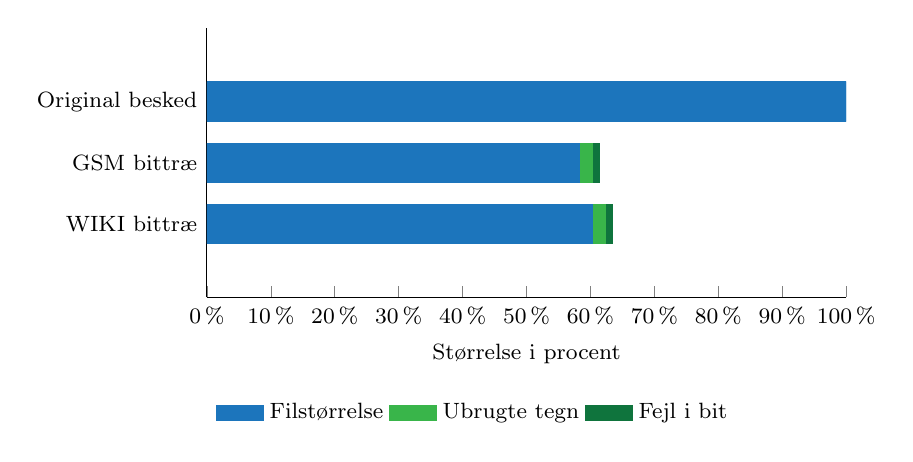
\begin{tikzpicture}
\begin{axis}[xbar stacked,
legend style={legend columns=4,at={(0,-0.35)},anchor=north west,draw=none},
ytick={0,1,2},
axis y line*=none,
axis x line*=bottom,
tick label style={font=\footnotesize},
legend style={font=\footnotesize},
label style={font=\footnotesize},
xtick={0,10,20,30,40,50,60,70,80,90,100},
width=.8\textwidth,
height=5cm,
bar width=5mm,
xlabel={Størrelse i procent},
yticklabels={WIKI bittræ, GSM bittræ, Original besked},
xmin=0,
xmax=100,
area legend,
enlarge y limits=0.6,
xticklabel=$\pgfmathprintnumber{\tick}$\,\%,
]
% Filstørrelse
\addplot[Sapphire,fill=Sapphire] coordinates
{(60.37,0) (58.34,1) (100,2)};
% Ubrugte tegn
\addplot[ForestLight,fill=ForestLight] coordinates
{(2,0) (2,1) (0,2)};
% Fejl i bit
\addplot[ForestGreen,fill=ForestGreen] coordinates
{(1.1,0) (1.1,1) (0,2)};
\legend{Filstørrelse,Ubrugte tegn, Fejl i bit}
\end{axis}
\end{tikzpicture}
\caption{Filstørrelse i forhold til original størrelse}
\label{resultatgraf}
\end{figure}


Som også ses på \ref{resultatgraf} er det gennemsnitligt lykkedes at komprimere en besked op til 42\% ved 
hjælp af det statiske bit-træ skabt ud fra SMS beskeder.
Her skal det så også pointeres at dette bit-træ er skabt ud fra disse SMS beskeder, så denne er netop optimeret 
til denne samling af SMS beskeder, hvorimod en ny samling, vil være en smule anderledes.

Ved at udregne ligningen X tegn * 0,6 = 160 tegn, hvor X er det antal tegn, som det er muligt 
gennemsnitligt at sende komprimeret. 0,6 er de 60\%, som det gennemsnitligt er muligt at mindske filens 
størrelse til. De 160 tegn, er det antal tegn, som der kan sendes med en SMS-besked.
Herved er det muligt at skrive op til 266 tegn i en enkelt SMS.


\chapter{Konklusion}

           Dette projekt omhandler tekstkomprimering og hvordan man kan bruge dette i forbindelse med SMS-beskeder, som har en øvre grænse for hvor mange tegn man kan sende pr. besked. Den første del af vores problemformulering lyder;
\emph{Hvordan kan man spare forbrugeren for dobbelt SMS-takst, ved brug af et komprimeringsprogram?}
Til at besvarer dette spørgsmål, hvar vi udviklet et program, som kan komprimere en tekstbesked ved brug af Huffman-algoritmen. Som det ses i afsnittet RESULTATER er det lykkedes af komprimere bedskeder med over 50 procent, hvilket betyder at det, med brug af programmet, er muligt at sende to SMS-beskeder som én. På den måde vil brugeren kunne spare SMS-takst, hver gang der skal sendes en SMS på over 160 tegn. 
Næste del af vores problemformulering lyder;
\emph{Hvordan kan man undgå at programmet bliver en belastning for brugeren?} og dette 



           \section{Perspektivering}
	Løsningen på problemet er som beskevet et komprimeringsprogram. Programmet komprimerer tekstbeskeder, så de fylder mindre og man på den måde kan sende flere tegn i den samme SMS. Når en SMS afsendes, sendes denne som en komprimeret tekststreng og som sådan vil den også modtages af modtageren af beskeden. Derfor kræver vores løsning at modtageren også har programmet. Hvis man som bruger sender komprimerede beskeder skal man være sikker på at motagerene af SMS-beskederne ligeledes har programmet, ellers giver beskeden ingen mening for dem. En løsning på dette problem, kunne være at lave en opdatering, med programmet, således at alle kunne opdatere deres mobiltelefon og derved have programmet. 

           \section{Det videre arbejde}
	Hvis vi skulle lave projeket igen, ville vi forsøge at indsamle data om interessenterne for løsningen. Det ville eksempelvis være interessant at vide hvor mange SMS'er de sender, både indenrigs og udenrigs. Derudover ville det selvfølgelig være vigtig at vide hvor mange af deres SMS-beskeder, der overstiger 160 tegn. Til at indsamle denne kvantitative data, ville en spørgeskema undersøgelse være en god mulighed. Ved at have denne data, kunne man regne på den faktiske besparelse på SMS-forbrug for et firma eller privat personer, hvis de implementerede vores software. Herved kunne vi vurdere om programmet ville have en effekt af betydning. 
På samme tid kunne det også være relevant at kigge på om vores software ville påvirke teleselskaberne og hvorvidt det ville være positivt eller negativt. Ville de miste penge ved at deres kunder sender færre SMS'er, eller ville de selv kunne spare penge hvis implementerede softwaren i deres netværk?
Derudover kunne man også undersøge hvor man ellers med fordel kunne bruge datakomprimering. Det kunne eksempelvis være når man skal lagre filer og ved generel internet trafik. Derved kunne vi finde ud af om vores software kunne være relevant i andre sammenhænge.

%\begin{thebibliography}{99} %Max
\bibliographystyle{plain}
\bibliography{Referencer}
%\end{thebibliography}

\begin{figure}[H]
\includegraphics []{Billeder/tegnsaet.png}
\caption {Her ses skemaet for bit 7 tegnsaettet. Ved 0x12 ses tegnet 1), der er et escape tegn til den ekstra tabel, som ses }
\label {tegnsaet}
\end{figure}

\begin{figure}[H]
\includegraphics []{Billeder/tegnsaet2.png}
\caption {Den ekstra tabel for bit 7 tegnsaettet}
\label {tegnsaet2}
\end{figure}


\end{document}

